\documentclass{beamer}
\setbeamertemplate{navigation symbols}{}

\title{ECE 417/598: Image formation}
\author{Vikas Dhiman}
\date{Feb 2, 2022}
\begin{document}
\begin{frame}
  \titlepage
  \end{frame}
\begin{frame}{Additional reference}
  Chapter 6, 7, 8 of  
  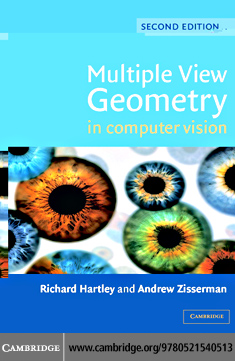
\includegraphics[width=0.3\linewidth]{media/hartley-and-zisserman.png}
  \footnote{Lookup on libgen.rs}
 \end{frame}
\begin{frame}
  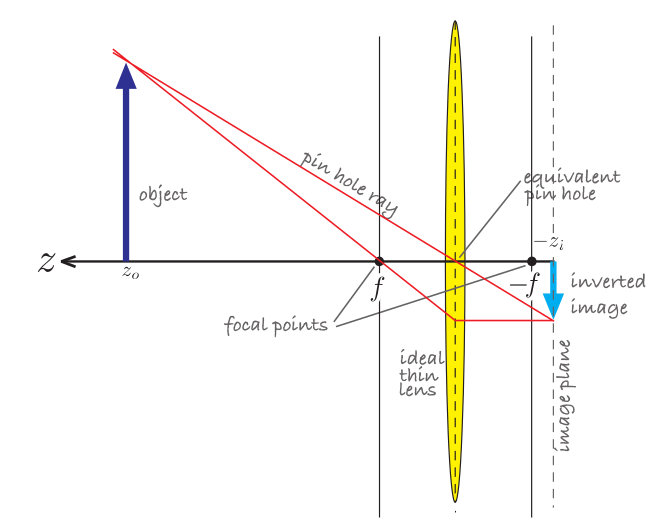
\includegraphics[width=0.48\linewidth]{media/lens-image-formation.png}
  \\
  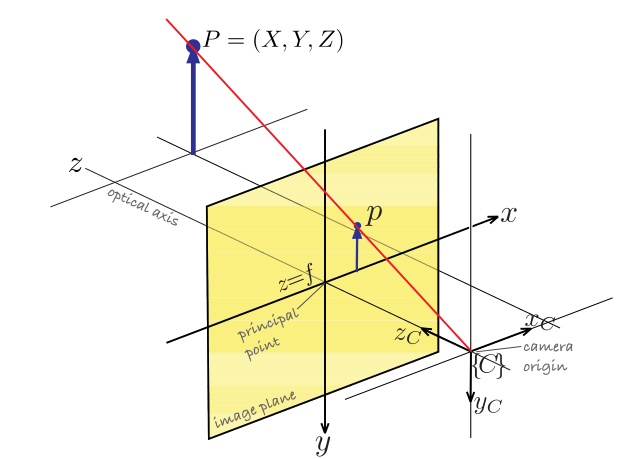
\includegraphics[width=0.48\linewidth]{media/pinhole-camera-model.png}
  \footnote{Chapter 11. Corke.}
\end{frame}
\begin{frame}
  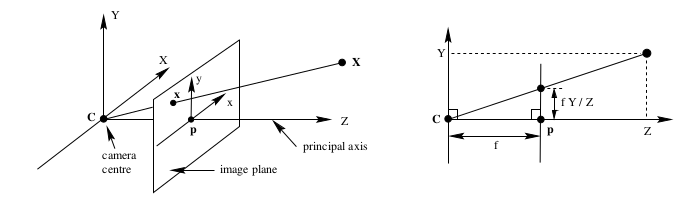
\includegraphics[width=\linewidth]{media/pinhole-camera-model-2.png}
  \footnote{Chapter 6. Hartley and Zisserman}
  \end{frame}
  \begin{frame}
    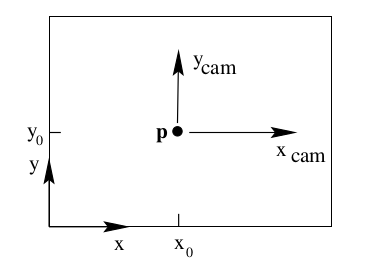
\includegraphics[width=0.4\linewidth]{media/image-center.png}
    \footnote{Chapter 6. Hartley and Zisserman}
  \end{frame}

  \begin{frame}
    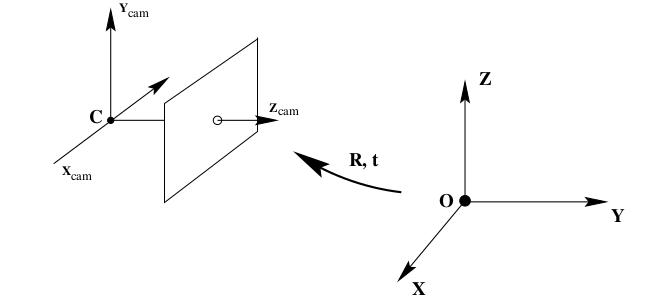
\includegraphics[width=0.4\linewidth]{media/world-camera-transformation.png}
    \footnote{Chapter 6. Hartley and Zisserman}
  \end{frame}

  \begin{frame}
    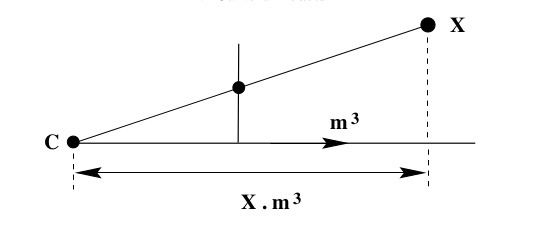
\includegraphics[width=0.4\linewidth]{media/recovering-ray-from-point.png}
    \footnote{Chapter 6. Hartley and Zisserman}
  \end{frame}

  \begin{frame}{A numerical example}
    Image is a grid of numbers. The vale in the grid represents intensity values.
    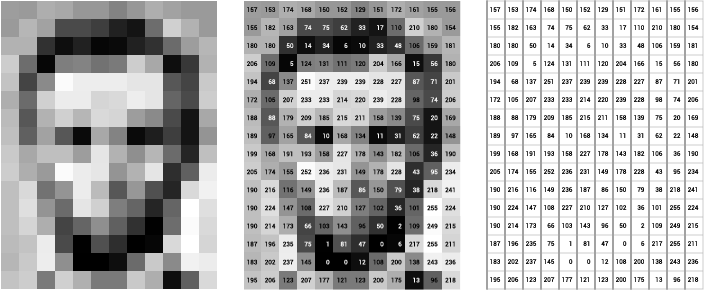
\includegraphics[width=\linewidth]{media/image-as-a-matrix.png}
  \end{frame}

  \begin{frame}
    A Depth Image is an array of numbers. The value in the grid represents
    intensity values.\\
    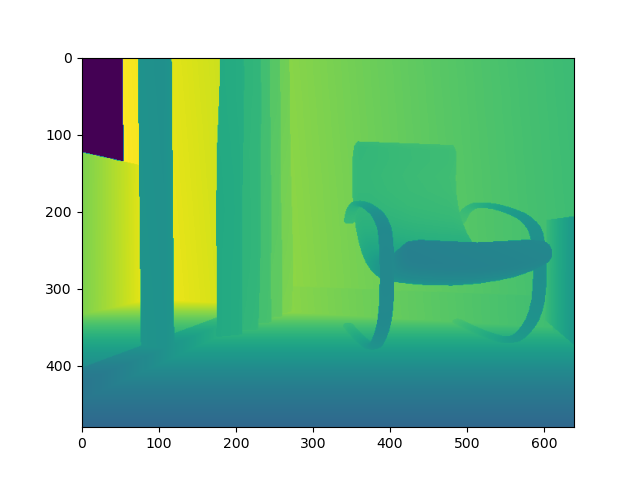
\includegraphics[width=0.45\linewidth]{media/00000-depth.png}%
    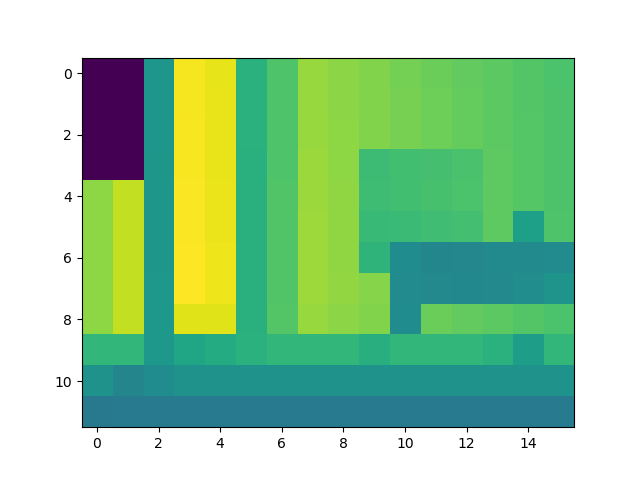
\includegraphics[width=0.45\linewidth]{media/00000-depth-lowres.png}
  \end{frame}

  
  \begin{frame}
    From what we have learned, how can we convert the depth image to a point cloud?
    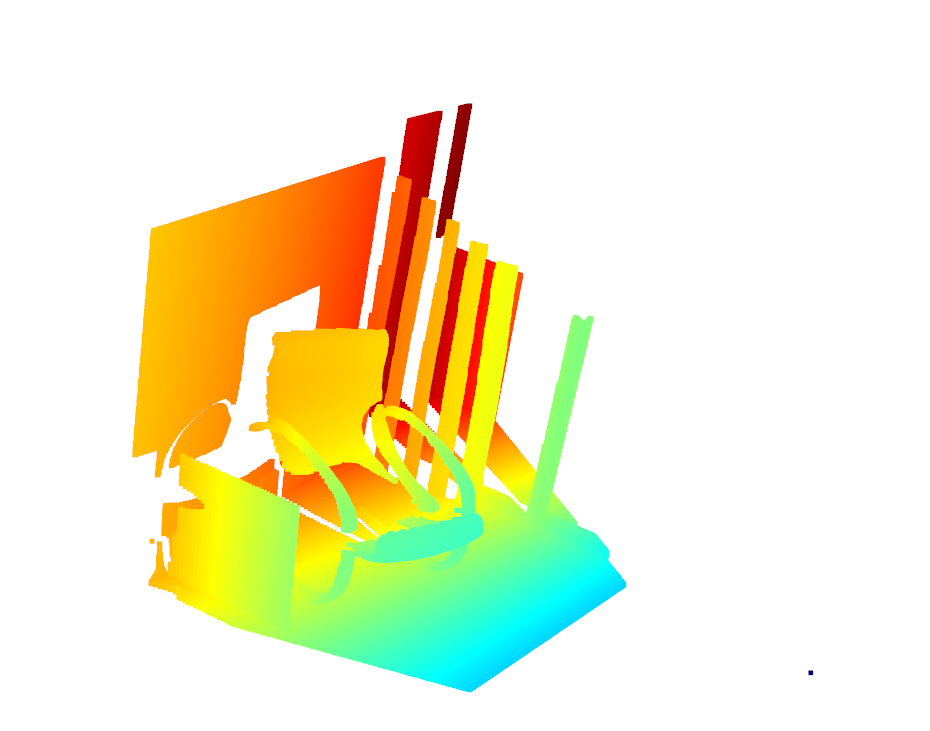
\includegraphics[width=0.45\linewidth]{media/depth-image-to-point-cloud-1.png}%
    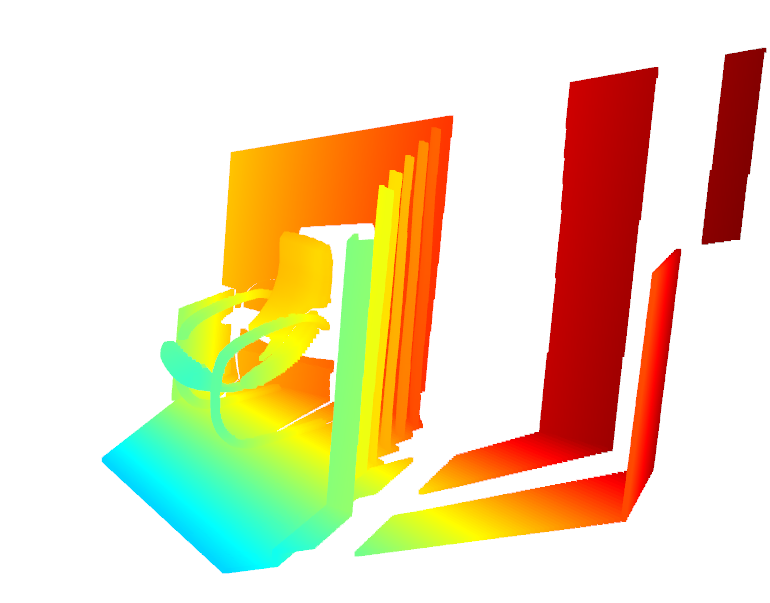
\includegraphics[width=0.45\linewidth]{media/depth-image-to-point-cloud-2.png}
  \end{frame}


  \begin{frame}{Pseudo-Inverse}

  \end{frame}

  \begin{frame}{Points as rays: aka Prospective geometry}
  \end{frame}

  \begin{frame}
    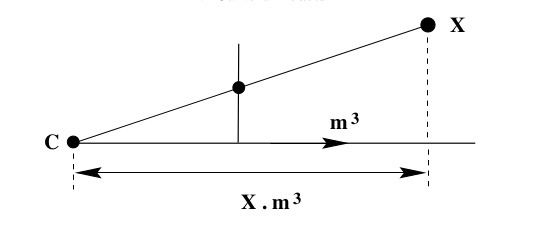
\includegraphics[width=0.4\linewidth]{media/recovering-ray-from-point.png}
    \footnote{Chapter 6. Hartley and Zisserman}
  \end{frame}

  \begin{frame}{Vanishing Point}
    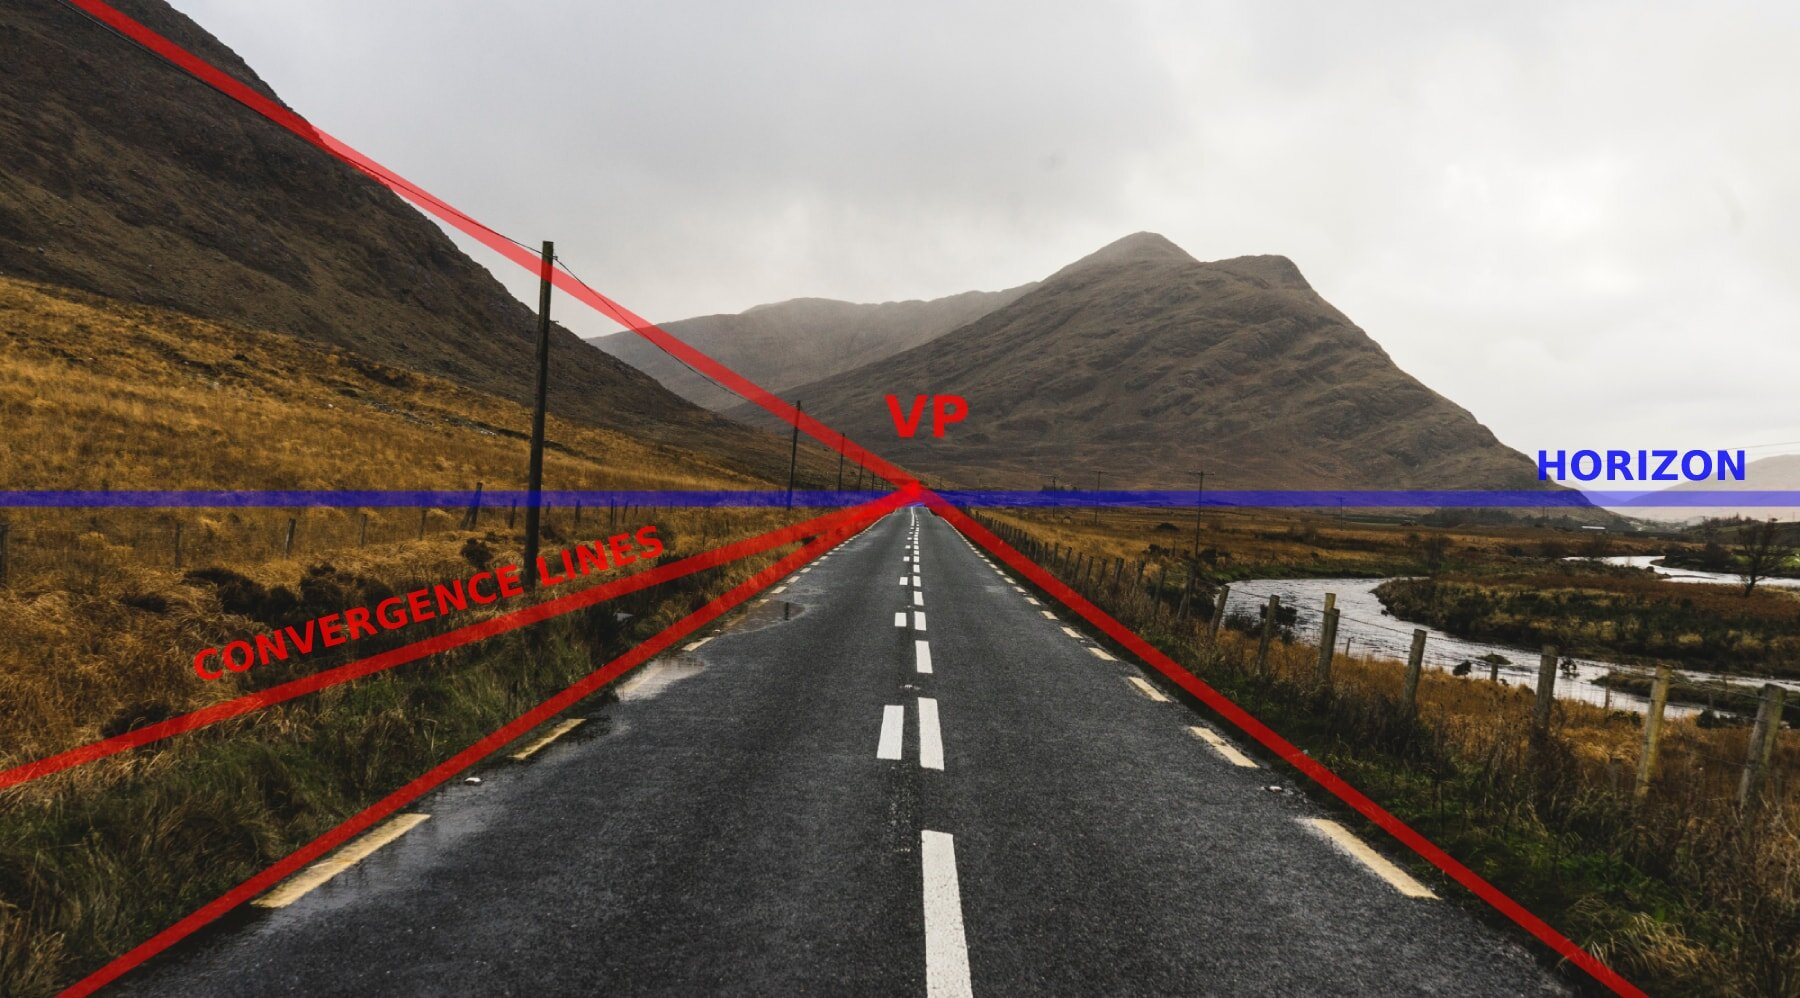
\includegraphics[width=0.7\linewidth]{media/vanishing-lines.jpeg}
    \\
    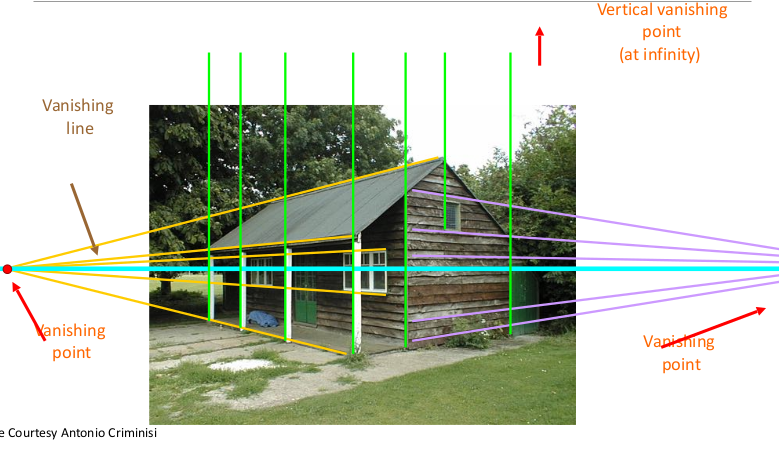
\includegraphics[width=0.7\linewidth]{media/vanishing-points.png}
  \end{frame}

  \begin{frame}{Vanishing Point}
    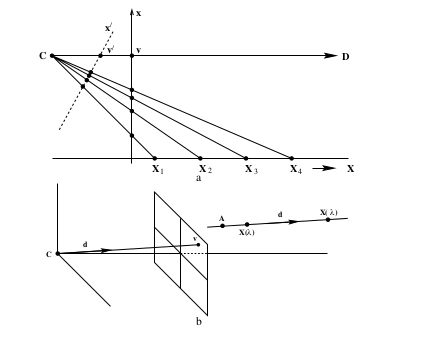
\includegraphics[width=0.5\linewidth]{media/vanishing-point-formation.png}
  \end{frame}

\end{document}